\documentclass[msc]{ppgccufmg}    % ou [msc] para disserta��es
                                  % de mestrado. Para propostas ou
                                  % projetos, usar [phd,project],
                                  % [msc,proposal], etc.

\usepackage[english]{babel}       % se o documento for em ingl�s
\usepackage[latin1]{inputenc}
\usepackage[T1]{fontenc}
\usepackage{type1ec}
\usepackage[a4paper,
  portuguese,
  bookmarks=true,
  bookmarksnumbered=true,
  linktocpage,
  colorlinks,
  citecolor=black,
  urlcolor=black,
  linkcolor=black,
  filecolor=black,
  ]{hyperref}
\usepackage[square]{natbib}


\usepackage{booktabs} % For formal tables
\usepackage[ruled]{algorithm2e} % For algorithms
\renewcommand{\algorithmcfname}{ALGORITHM}
\SetAlFnt{\small}
\SetAlCapFnt{\small}
\SetAlCapNameFnt{\small}
\SetAlCapHSkip{0pt}
\IncMargin{-\parindent}

\usepackage{graphicx}
\usepackage{mathtools}
\usepackage{amsfonts}
\usepackage{multirow}

\DeclareMathOperator*{\argmax}{arg\,max\,}
\renewcommand{\arraystretch}{1.2}

\begin{document}

\ppgccufmg{
  title={Web data extraction through named entity labeling},
  authorrev={de Freitas Veneroso, Jo�o Mateus},
  cutter={D1234p},
  cdu={519.6*82.10},
  university={Federal University of Minas Gerais},
  course={Computer Science},
  portuguesetitle={Extra��o de dados da web por rotulamento de sequ�ncias},
  portugueseuniversity={Universidade Federal de Minas Gerais},
  portuguesecourse={Ci�ncia da Computa��o},
  address={Belo Horizonte},
  date={2019-07},
  advisor={Berthier Ribeiro-Neto de Ara�jo},
  approval={pics/approvalsheet.eps},
  abstract=[brazil]{Resumo}{resumo},
  abstract={Abstract}{abstract},
  dedication={dedicatoria},
  ack={agradecimentos},
  epigraphtext={Truth and lie are opposite things.}{Unknown},
  keywords={Vis�o Computacional, Redes, Sabotagens},
}


% Os tr�s comandos seguintes s�o apenas para gerar texto para ocupar espa�o nas
% p�ginas.
\newcommand{\dummytxta}{%
Lorem ipsum dolor sit amet, consectetur adipisicing elit, sed do
eiusmod tempor incididunt ut labore et dolore magna aliqua. Ut enim ad
minim veniam, quis nostrud exercitation ullamco laboris nisi ut
aliquip ex ea commodo consequat. Duis aute irure dolor in
reprehenderit in voluptate velit esse cillum dolore eu fugiat nulla
pariatur. Excepteur sint occaecat cupidatat non proident, sunt in
culpa qui officia deserunt mollit anim id est laborum.\par
}

\newcommand{\dummytxtb}{%
Sed ut perspiciatis unde omnis iste natus error sit voluptatem accusantium
doloremque laudantium, totam rem aperiam, eaque ipsa quae ab illo inventore
veritatis et quasi architecto beatae vitae dicta sunt explicabo. Nemo enim
ipsam voluptatem quia voluptas sit aspernatur aut odit aut fugit, sed quia
consequuntur magni dolores eos qui ratione voluptatem sequi nesciunt. Neque
porro quisquam est, qui dolorem ipsum quia dolor sit amet, consectetur,
adipisci velit, sed quia non numquam eius modi tempora incidunt ut labore et
dolore magnam aliquam quaerat voluptatem. Ut enim ad minima veniam, quis
nostrum exercitationem ullam corporis suscipit laboriosam, nisi ut aliquid ex
ea commodi consequatur? Quis autem vel eum iure reprehenderit qui in ea
voluptate velit esse quam nihil molestiae consequatur, vel illum qui dolorem
eum fugiat quo voluptas nulla pariatur?\par
}

\newcommand{\dummytxtc}{%
At vero eos et accusamus et iusto odio dignissimos ducimus qui blanditiis
praesentium voluptatum deleniti atque corrupti quos dolores et quas molestias
excepturi sint occaecati cupiditate non provident, similique sunt in culpa qui
officia deserunt mollitia animi, id est laborum et dolorum fuga. Et harum
quidem rerum facilis est et expedita distinctio. Nam libero tempore, cum soluta
nobis est eligendi optio cumque nihil impedit quo minus id quod maxime placeat
facere possimus, omnis voluptas assumenda est, omnis dolor
repellendus. Temporibus autem quibusdam et aut officiis debitis aut rerum
necessitatibus saepe eveniet ut et voluptates repudiandae sint et molestiae non
recusandae. Itaque earum rerum hic tenetur a sapiente delectus, ut aut
reiciendis voluptatibus maiores alias consequatur aut perferendis doloribus
asperiores repellat.\par
}

\newcommand{\dummytxt}{\dummytxta\dummytxtb\dummytxtc}

\chapter{Introduction}

HTML documents most often lie in between the structured/unstructured 
data paradigm. DOM hierarchy, element disposition, CSS classes, and other 
features related to the document structure and indirectly associated with the 
data itself can be valuable information on the task of identifying
entities. Yet, we cannot expect these features to be completely constrained 
by an underlying pattern. Organization patterns tend to follow some guidelines 
but they are in no way subject to strict rules. That is why classical web data 
extraction systems such as automatic wrapper generators 
\cite{Kushmerick2000,Hsu1998,Muslea1999}
do not translate very well across different websites. 

Most existing Web data extraction methods are tailored to extract data 
from a single webpage, producing different compromises between efficacy and 
degree of human supervision. Some unsupervised approaches proposed to tackle 
the problem of data extraction for whole application domains 
\cite{Zhu2005,Zhu2006,Abdessalem2010,Furche2012,Furche2012a}. Usually, 
unsupervised WDE methods work in two stages. In the record segmentation stage,
WDE systems seek to cluster visually and structurally similar webpage regions 
and identify repeating data records with heuristics and 
hand-coded rules. In the attribute labeling stage, WDE systems seek to identify 
the correct attributes on data records, many times resorting to regular expressions 
or gazetteer matching strategies. The outcome of each of these stages can aid one 
another. The inner patterns of data records can help in identifying attributes of other 
data records. Also, by properly identifying data record attributes, it becomes 
easier to determine boundaries and perform record segmentation.

While unsupervised approaches can be sometimes adequate to extract information from 
webpages with similar templates, they usually fail on cross-website data extraction 
tasks. Also, more sophisticated approaches may be needed when we are not dealing
with easily distinguishable attributes such as prices and dates. In this regard, 
machine-learning-based sequence labeling methods can provide a more flexible 
approach that works regardless of website structure.

In recent years, we saw an amazing progress in the field of Natural Language Processing, 
particularly with the introduction of deep recurrent neural network architectures
for sequence labeling. However, despite Web data extraction being a closely 
related field, there is a lack of extraction tools that make use of these recent 
advancements. The attribute labeling stage in Web data extraction systems
is essentially a Named Entity Recognition (NER) problem, the problem of 
detecting named entities in the text and classifying them into predetermined 
categories such as person names, locations, dates or organizations. 

In many cases, such as when we are extracting researcher names from faculty listings,
detecting named entities is sufficient to solve the data extraction task. However, when we are
dealing with multi-attribute data records or complex relationships, we may need to 
perform additional steps. Nevertheless, even in the latter cases, flexible NER methods 
are still desirable because, while many WDE algorithms can effectively exploit the 
semi-structured nature of Web documents, too much reliance on structural webpage 
features often produce poor generalizations on cross website extraction. Also, 
data records may enclose plain text with relevant named entities. 

In this article, we investigate methods of named entity recognition for Web data extraction.
Recently proposed neural architectures have achieved exciting results 
on the NER task in plain text while requiring almost 
no feature engineering or access to gazetteers \cite{Huang2015,Lample2016,Ma2016}. 
NER on HTML poses a slightly different type of challenge. Named entities may occur inside 
tables, lists, or other types of visual elements that provide little to no textual 
information that could give hints about the semantic category of a word. Still, even 
with this limitation, we show that it is possible to obtain very good results with a 
relatively small training set.

By reliably detecting named entities on HTML, we can improve the performance of existing WDE 
approaches or even construct an end-to-end neural network architecture to solve domain 
wide data extraction with considerable flexibility. To test different NER approaches to
Web data extraction, we explored the task of researcher name extraction from university 
faculty listings across the world, introducing a novel NER dataset.

Reliable researcher affiliation information is often missing from public researcher 
databases (especially in departments other than Computer Science). Also, the display of 
faculty information varies significantly between different university websites, so 
this task can provide a good measure of the expected performance and data need of
NER methods on other Web data extraction tasks. 


\chapter{Problem Definition}

Web data extraction is a task that is constituted of many overlapping
problems that demand integrated and sophisticated solutions. Most often, information
extraction tools that work exceptionally well on a given task end up performing poorly 
when given even a slightly different task. Traditional methods of web data extraction
were mainly concerned with the extraction of entities described by a simple ontology
from web pages generated by the same source (e.g. collecting house prices and addresses 
from real estate portals). The extraction of complex entities from a plethora of sources 
presents a different class of problems. The former case could be solved by rigid tools
with hard coded rules that many times yielded close to perfect results. The latter case,
however, demands far more flexible approaches since the extraction tools are required to 
deal with a greater variety of page arrangements and also with entities that are ambiguously 
defined. In many aspects, the flexible extraction of entities from web pages is more similar 
to the tasks of named entity recognition and relationship extraction from plain text than 
to the tasks that concerned the early information extraction methods.

Recent advancements in sequence models for natural language led to important 
breakthroughs in applications such as speech recognition, machine translation, 
sentence segmentation, and sequence labeling (which concerns us more directly). 
In fact, if we treat all sentences in a web page as sequences extracted from an 
underlying presentation graph (i.e. the DOM tree), the problem of information 
extraction can be solved through the consecutive application of three NLP tasks: 
sentence segmentation, named entity recognition, and relationship extraction. 
First, we need to segment the relevant grouping structures (e.g. sentences, rows in table, 
items in a list). Then, we must identify relevant named entities (e.g. person names,
companies, locations). And finally, we have to discover the relationships between 
those named entities (e.g. person X works in company Y). The work flow is the same
for plain text and web pages, but there are important differences chiefly related
to the structure of the data or the lack of it.

In this dissertation, we investigate the best methods for sequence labeling on HTML. 
To evaluate these methods, we assess their performance on the task of researcher 
name extraction from faculty directories of universities across the world.
We will be mainly concerned with the task of named entity recognition but a brief
discussion of the challenges involved in the task of sentence segmentation for HTML 
will be provided in Chapter~\ref{sec:dataset}. The task of relationship extraction,
however, is not relevant to the problem of researcher name extraction and will not be
discussed. 

The remainder of this chapter will describe in more depth the subject of this dissertation.
Section~\ref{sec:web_data_extraction} discusses the task of Information Extraction in the Web.
Section~\ref{sec:named_entity_recognition} discusses the importance of Named Entity Recognition 
for Web Data Extraction. 
Finally, Section~\ref{sec:researcher_name_extraction} describes the specific problem 
of Researcher Name Extraction.

\section{Information Extraction in the Web}
\label{sec:web_data_extraction}

\textit{Information Extraction} consists of mapping unstructured or poorly structured 
data to a semantically well defined structure. "(It) is the process of filling the fields and 
records of a database from unstructured or loosely formatted text"~\cite{McCallum2005}. 
Usually, the input consists of a corpus containing useful entities that
are scattered in the text and the information extraction system is responsible
for finding these entities and organizing them according to a rigid hierarchy such as
the one defined by the schema of a relational database. It must be stated that it is somewhat
misleading to refer to plain text as unstructured data, since prose has a loosely defined structure 
that ultimately renders it comprehensible. However, in the context of \textit{Information Extraction} 
we refer to unstructured data in contraposition to tabular data, which are in many cases 
easier to work with than plain text.

\textit{Information Extraction} is a multifaceted problem that spans communities 
of researchers in the fields of \textit{Text Mining}, Information Retrieval, and Natural 
Language Processing. \textit{Text mining} is the search of patterns in unstructured text 
that may involve document clustering, document summarization, \textit{Information Extraction},
and other subtasks. \textit{Information Retrieval} is tipically concerned with the parsing, 
indexing and retrieval of documents and \textit{Information Extraction} can help giving a more precise 
answer to the user's information needs. Finally, \textit{Natural Language Processing}
is a field of Computer Science concerned with how computers process and understand natural 
language of which two subtasks, namely Named Entity recognition and Relation Extraction,
are of special importance for \textit{Information Extraction}.

A popular application of \textit{Information Extraction} is the identification of 
entities such as people, organizations, or events from news sources and the determination
of their relations. For example, one could be interested in determining who is the CEO of a company
that was mentioned in the news or which politicians support a bill that is being considered
by the Congress. Another interesting news-related application of \textit{Information Extraction} 
is tracking disease outbreaks through the extraction of disease names and locations 
from news sources and determining their relation to outline the geographical area affected 
by an epidemy (cite example). Other \textit{Information Extraction} systems proposed 
to track disease outbreaks through the analysis of tweets (cite example), which presents a 
remarkably different challenge since the context of tweets is very limited and the presence
of abbreviations and typos is more widespread than in the case of highly curated content
such as news.

The field of bio-informatics has also found important applications for 
\textit{Information Extraction}. The first BioCreAtIvE challenge dealt with extraction 
of gene or protein names from text, and their mapping into standardized gene identifiers 
for three model organism databases (fly, mouse, yeast).~\cite{Hirschman2005}.
In the BioCreative/OHNLP Challenge 2018~\cite{Rastegar-Mojarad2018}, researchers 
were required to investigate methods of family history information extraction. Family
history is a critical piece of information in the decision process for diagnosis and 
treatment of diseases, however the main sources of data are unstructured electronic 
health records. The task is divided in two subtasks: 1) Entity recognition 
(family members and disease names); and 2) Relation Extraction (family members and
corresponding observations).

Another scientific application for \textit{Information Extraction} methods is the 
the extraction of information from research papers to populate citation 
databases and bibliography search engines such as Citeseer~\cite{Lawrence1999}, 
DBLP~\footnote{http://dblp.uni-trier.de/}, 
Semantic Scholar~\footnote{https://www.semanticscholar.org}, and 
Google Scholar~\footnote{https://scholar.google.com/}.
The vast amount of scientific knowledge produced daily demands automatic
methods for extracting authors, titles, affiliations, references, venues 
and the year of publication from research papers and online resources such
as university websites, individual researcher home pages and conference
websites. This application is especially important to the evaluation and 
bibliometrics research communities, that are concerned with the measure of
academic impact and researcher productivity through the usage of quantitative
indices of academic impact such as the H-index~\cite{Hirsch2005} and 
P-score~\cite{Ribas2015a}. 

\textit{Web Data Extraction} works a little different from
\textit{Information Extraction} in plain text because HTML documents frequently
lie in between the structured/unstructured data paradigm. Relevant entities 
may occur inside tables, lists, or other types of visual elements that provide 
little to no contextual information that could give hints about their category.
Web pages have a two dimensional tabular structure that is usually more similar
to a spreadsheet than to text found in news corpora. For this reason, features
extracted from the DOM hierarchy such as element disposition, CSS classes, and
nesting structure can provide valuable information in identifying entities and
extracting their attributes. Yet, we cannot expect these features to be completely 
constrained by an underlying pattern. Organization patterns tend to follow some 
guidelines but they are in no way subject to strict rules. 

Most existing Web data extraction methods are tailored to extract data 
from a single webpage, producing different compromises between efficacy and 
degree of human supervision. Usually, these methods work in two steps. In the 
record segmentation step, we seek to cluster visually and structurally 
similar webpage regions and identify repeating data records. In the attribute 
labeling stage, we seek to identify the correct attributes for each data record,
maybe resorting to regular expressions or simple dictionary matching strategies
depending on the task at hand. The outcome of each step can aid one 
another. The inner patterns of data records can help identifying attributes 
of other data records. Also, by properly identifying attributes, 
it becomes easier to determine boundaries and perform record segmentation 
correctly. Figure~\ref{fig:amazon} shows how a hypothetical \ref{Web Data Extraction} 
system that aims to collect book titles and prices from Amazon could perform record
segmentation and attribute labeling.

The task of extracting product names and prices from online catalogs can 
likely be solved by a rather inflexible system that operates mainly with 
hard coded rules and simple regular expressions, especially if we only 
consider pages with a very similar template (e.g. Amazon product listings).
Classical wrapper generators \cite{Kushmerick2000,Hsu1998,Muslea1999} are 
well suited for this type of task. However, when we need to identify more 
complex and ambiguous entities such as researcher names in many different 
contexts such as faculty websites, we might be better off with a more 
flexible approach. The task of Named Entity Recognition aims to identify
named entities (e.g. people, organizations, etc.) in plain text, but we will
see in the next chapters that the sequence models that work well in plain text
can also be employed succesfully in web extraction tasks, sometimes with a few
alterations.

This section gives a brief introduction to \textit{Information Extraction}, but
there are many applications that were not discussed here. A more detailed view 
of the field is given in Sarawagi~\cite{Sarawagi2008}.

\section{Named Entity Recognition}
\label{sec:named_entity_recognition}

\textit{Named Entity Recognition} is a task in Natural Language Processing that
aims to identify \textit{Named Entities} in a text. The Named Entity Recognition 
task first appeared as a subtask of 
\textit{Information Extraction} in the context of the Message Understanding 
Conference (MUC) promoted by the american Naval Ocean Systems Center. In 
MUC-3, a precursor task involved extracting information on terrorist 
incidents (incident type, date, location, perpetrator, target, instrument,
outcome, etc.) from messages disseminated by the Foreign Broadcast
Information Service of the U.S. Government~\cite{Sundheim1991}. In MUC-6~\cite{Grishman1996} the 
"named entity" task was created with the goal of identifying the names of people, 
organizations, and geographic locations from articles of the Wall Street Journal.
In MUC-7, the task was expanded to handle multilingual evaluation and 
"Named Entities (NE) were defined as proper names and quantities of 
interest. Person, organization, and location names were marked as well 
as dates, times, percentages, and monetary amounts"~\cite{Chinchor1998}.
The shared-task at the Conference on Computational Natural Language Learning 
in 2003~\cite{KimSang2003} concerned language-independent named entity recognition 
and it is especially important because it established an enduring data format for
NER and it introduced a dataset of articles extracted from news sources that is to this
day still employed to evaluate the quality of NER systems.

The task of \textit{Named Entity Recognition} is essentialy a sequence labeling
task. That is, given a sequence of tokens we want to attribute labels to each
token classifying them in one of a number of predefined classes. Figure~\ref{fig:ner_example}
describes the process of atributing Named Entity labels to a sentence according to the
CONLL format. There are cases where a token may belong to more than one class because of
nested named entities (e.g. in "CoNLL 2003", 2003 is both part of a conference name and a date).
This complexity is of importance to some applications~\cite{Katyar2018} but it will not be discussed 
here because nested named entities are absent from our concrete problem of researcher name extraction
and most sequence models can be adapted to handle this special case with a few modifications.

A simple approach to \textit{Named Entity Recognition} can be devised through the use
of regular expressions, that are search patterns that describe a regular language and which can
be easily implemented in most programming languages. These programs can be perfectly suited
to extract regular entities such as dates and prices with almost perfect accuracy. The extraction
of other types of entities that belong to a limited set such as the names of states in a country can 
be accomplished through dictionary matching. Other types of entities such as the ones investigated in
the CoNLL-2003 challenge require more sophisticated methods of sequence labeling.

Some classical statistical methods of \textit{Sequence Labeling} that are able to handle the labeling
of complex entities with decent accuracy are Hidden Markov Models, Linear Chain 
Conditional Random Fields and Maximum Entropy Markov Models. The first two will be explored
in further detail in Chapter~\ref{cha:sequence_models}, and the latter is essentialy a more
restrictive discriminative model in comparison to Condition Random Fields. These statistical 
approaches have had remarkable resiliency in \textit{Sequence Labeling} tasks and still provide 
a good first approximation to a solution because of their simplicity, speed and accuracy.

The deep learning revolution has brought huge advancements to \textit{Named Entity Recognition}, 
as was the case with most NLP tasks. Deep learning differs from classical machine learning in
regard to the levels of abstraction learned by the classifiers. Deep learning techniques combine 
feature extraction and classification in a single system. While a conventional feed-forward
neural network may perform classification by learning the weights of a single hidden layer through
backpropagation, a deep learning model is usually composed of multiple hidden layers that handle 
different levels of abstractions. In text related tasks, the first level of abstraction could
consist of a word embedding layer, where words are mapped to a continuous vectorial space with
reduced dimensionsality, and the next level of abstraction could be composed of a multi layered 
recurrent neural network. 

Essentialy all the best scoring models at the Conll-2003 task employ some form of deep 
neural network, and most often Long Short Term Memory 
recurrent neural networks with a range of differing characteristics. When combined with pretrained
word embeddings these models provide a powerful method of sequence labeling that requires 
practically no feature engineering or dictionary matching. However, these models have 
become quite complex, constrasting with earlier approaches such as Hidden Markov Models, that
only require estimation of a comparatevely small number of weights in closed form. The training time
required by such deep models is many orders of magnitude larger than that of classical approaches, 
and if we take into consideration the training of word embeddings such as Word2Vec's skip gram model 
in a billion token corpus, it is no exaggeration to say that deep learning models increase the 
training time a thousandfold when compared to earlier approaches. Additionaly, most deep learning 
models require expensive hardware in the form of GPUs or 
TPUs~\footnote{Those are Google's Tensor Processing Units "https://cloud.google.com/tpu/"}
to become practical options. 

Despite some noteworthy efforts on data visualization {references here}, DNNs still lack 
interpretability. Also, they have limited applicability when we care about causal inference 
{references here}, a goal that is especially meaningful in applied statistics and the social 
sciences. Regardless, it must be acknowledged that deep learning is a remarkably useful tool to build 
classifiers with unparallaled accuracy in \textit{Named Entity Recognition} as well as in other
tasks. We must only be aware of its shortcomings.

\section{Researcher Name Extraction}
\label{sec:researcher_name_extraction}

This dissertation has the goal of finding the best approaches to sequence modelling for 
Web Data Extraction. To achieve this goal, we compare multiple systems at the researcher 
name extraction task. The task consists of extracting researchers names from university 
faculty listings across the world to discover their affiliations and link their profiles 
to public databases such as DBLP or Google Scholar~\footnote{
  This is useful, for instance, if one needs to compare the research output of 
  deparments in Germany, or study international publication patterns.
}. Public researcher databases only have sparse information about author affiliation and 
even in fields for which the information is more easily available, such as Computer Science,
only a small fraction of the records have reliable affiliation information. 

\begin{figure}
  \centering
  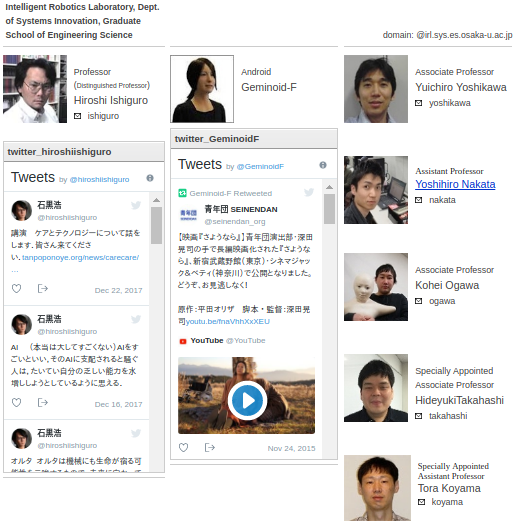
\includegraphics[width=1.0\textwidth]{pics/jap_osaka_lab}
  \caption{Example of a faculty directory}
  \label{fig:faculty_directory}
\end{figure}

To acknowledge the complexity of this task, take for example a snippet extracted from
the staff page for the intelligent robotics laboratory from Osaka University shown in 
Figure~\ref{fig:faculty_directory}. There is some structure to the way member profiles are arranged, 
but the organization is rather flexible. Other pages, even from the same website, can show very different 
patterns, ranging from tables and lists to free form.
Researcher names can appear inside plain text, similar to the case of \textit{Named Entity Recognition}
from news sources or in a more tabular structure. Names may also be part of larger sentences such as in 
"Michael Johnson Chair" and "John Doe Avenue" yielding false positives. Or they can be composed 
of common words (e.g. Summer Hall) yielding false negatives. There is no rule that fits all cases.

State-of-the-art named entity recognition models trained on news datasets (cite here) do not
perform so well at this task, because in many webpages, text alone is insufficient to provide proper 
contextual information about the semantic category of a word. The absence of context demands
extraction systems to rely on information from sources outside the dataset, being them 
features extracted from unlabeled corpora obtained through unsupervised pretraining, or 
dictionaries containing many instances of the relevant entities. Although, entity instances will rather 
frequently be unique occurences, rendering dictionary matching approaches
insufficient. Therefore, a key problem in the task of entity name extraction is accounting for all
possible name combinations, even those that seem unlikely. Since there is no database with all 
possible named entity combinations, we need holistic statistical methods that can handle 
unknown tokens with relative efficacy.

Considering that NER datasets built from news corpora such as CoNLL-2003 do not provide an adequate 
measure for the performance of sequence models on HTML, we introduce the NER-on-HTML dataset
to evaluate the performance of different sequence models at the researcher name extraction task. 
This dataset is described in Chapter~\ref{cha:dataset}.

Another important related task in the context of researcher name extraction is performing named 
entity disambiguation, which consists of linking the extracted named entities to a unique profile in a 
unified database. This task is called \textit{Named Entity Linking}. Roughly half the records found in 
faculty webpages can be linked to their records in public databases without great difficulty. For the 
other half we may need to employ more complex systems or perform manual classification. This task 
however is not the object of our study.

\chapter{Dataset}
\label{cha:dataset}

This chapter describes the dataset used to evaluate the performance of sequence models
on the Web data extraction task. We call it the NER-on-HTML dataset. The task consists 
of finding researcher names in faculty listings from university webpages across the world,
mainly from Computer Science departments.
This would be a
necessary step when linking researcher profiles from university websites to their entries
in public databases such as DBLP \footnote{http://dblp.uni-trier.de/}. Unlike many
information extraction datasets, each webpage in the dataset comes from a different 
website, and therefore has a different format, what makes many information
extraction approaches impractical. The idea is to explore systems that are general 
enough to allow efficient entity extraction from different sources while requiring
no supervision between different websites. 

This task is similar to labeling authors in comments or articles collected
from different publishing platforms. Another similar task is NER on tweets.
Because of the character limitation, tweets rarely provide sufficient context
for NER systems to perform token labeling adequately.

We collected 145 computer science faculty pages from 42 different countries in
multiple languages, although the English version was preferred when it was available.
We gathered faculty webpages randomly in proportion to
the number of universities in each country\footnote{A detailed list of universities can
be found in https://univ.cc/world.php}. Each HTML page was preprocessed and converted
to the CoNLL 2003 data format. That is, one word per line with empty lines representing
sentence boundaries. Sentence boundaries were determined by line break HTML tags
(div, p, table, li, br, etc.) in contrast to inline tags (span, em, a, td, etc.). 
Sentences that were more than fifty tokens long were also split according to the
punctuation. The algorithm used for sentence segmentation is described in detail in
Appendix~\ref{app:html_segmenter}.

A proper HTML segmenter poses many challenges by itself. We wanted to evaluate 
models without relying on any sophisticated data record segmentation system.
In many cases, entity annotation may precede the segmentation
phase on Web Data Extraction methods. Also, depending on the task (as is the case
for researcher name extraction), a good annotator that is able to work 
with raw HTML allows for a more flexible system and can provide a sufficient 
solution.

Finally, all tokens were tagged using the IOB scheme put forward by
Ramshaw and Marcus \cite{Ramshaw1999} that is described in Figure~\ref{fig:iob}. 
The performance of sequence models in the NER-on-HTML dataset was evaluated 
according to the precision, recall and F-measures~\cite{Rijsbergen1979} in the test
set. Precision accounts for the percentage of named entities found by the model that are 
correct, this is the proportion of 
true positives relative to all extracted entities. Recall is the percentage of named entities 
that are present in the corpus and were found by the model, this is the proportion of true 
positives relative to all named entities that should have been extracted. The relation between
both of these measures is expressed in Figure~\ref{fig:precision_recall}. The F-measure score 
is a composite measure that combines precision and recall with the formula:

\begin{equation}
F_{\beta} = (1 + \beta^2) \cdot \frac{precision \cdot recall}{(\beta^2 \cdot precision) + recall}
\end{equation}

The choice for $ \beta $ depends on the importance attributed to the precision and recall measures.
This formula "measures the effectiveness of retrieval with respect to a user who attaches 
$ \beta$ times as much importance to recall as precision"~\cite{Rijsbergen1979}. A common choice
for the value of $ \beta $ is $ 1 $, this measure is called the $ F_1 $-score. That is, we attribute 
as much importance to recall as to precision.

\section{Data Description}

\begin{table}[h]
  \small
  \begin{center}
    \begin{tabular}{ lllll }
      \toprule
      Data file & Documents & Sentences & Tokens & Names \\
      \midrule
      Training    & 85  & 24728 & 110269 & 5822  \\  
      Validation  & 30  & 8743  & 36757  & 1788  \\
      Test        & 30  & 10399 & 44795  & 2708  \\
      \midrule
      Total       & 145 & 43870 & 151821 & 10318 \\
      \bottomrule
    \end{tabular}
  \end{center}
  \caption{Description of the data files in the NER-on-HTML dataset}
  \label{tab:dataset}
\end{table}

The NER-on-HTML dataset is comparable in size to other popular NER datasets.
It was divided in training, validation and test sets, which are described in 
Table~\ref{tab:dataset}. The validation set was used in the early stopping 
validation strategy to avoid overfitting classifiers, and model performance 
was evaluated by comparing the performance in the test set. 

Most web pages in this dataset are faculty directories with informative
text from small passages, eventhough prose is not absent from more than a few
webpages. Size and structure varies wildly, therefore some documents 
may contain up to a few hundred names whereas other documents may contain 
only twenty or thirty names. This difference in document size may be problematic
when comparing different extraction systems, because a system that performs well 
on pages with large content may perform poorly in a set of smaller pages, but this
characteristic would not affect so much the averaged results. A different approach 
might be to consider the averaged precision, recall and F-measures per page, 
privileging systems that have a more regular performance between websites. However, 
this approach might cover other deficiencies, since a system that produced 100 false 
positives in a page with 500 names would account for the same level of drop in average 
recall as a system that missed 10 false positives in a page with 50 names. For that
reason, we chose to keep the same criteria of evaluation used on other 
\textit{Named Entity Recognition} tasks, that is, calculating global precision, recall,
and F-measures relative to the total amount of named entties in the corpus.

\section{Differences between NER-on-HTML and ConLL-2003}

\begin{table}[h]
  \small
  \begin{center}
    \begin{tabular}{ llllllll }
      \toprule
      Data file & Documents & Sentences & Tokens & LOC & MISC & ORG & PER \\
      \midrule
      Training    & 946  & 14987 & 203621 & 7140 & 3438 & 6321 & 6600 \\  
      Validation  & 216  & 3466  & 51362 & 1837 & 922 & 1341 & 1842  \\
      Test        & 231  & 3684  & 46435 & 1668 & 702 & 1661 & 1617  \\
      \midrule
      Total       & 1393 & 22137 & 301418 & 10645 & 5062 & 9323 & 10059 \\
      \bottomrule
    \end{tabular}
  \end{center}
  \caption{Description of the CoNLL-2003 English dataset}
  \label{tab:conll}
\end{table}

The CoNLL-2003 dataset was introduced in the \textit{Named Entity Recognition} 
shared-task at the Conference on Computational Natural Language Learning and
is still one of the most popular NER datasets, being used to attest the performance
of state-of-the-art sequence labeling systems. The English data is composed of 
news stories extracted from the Reuters Corpus, and provides annotations for
four types of entities: people (PER), organizations (ORG), locations (LOC),
and miscellaneous (MISC), which includes entities that cannot be classified 
in one of the former groups. In this section, we present a brief 
comparison between the ConLL-2003 English dataset and the NER-on-HTML dataset to 
understand how documents from both sources differ, and why this difference may be 
responsible for the observed drop of performance when we apply NER systems trained 
in news corpora to HTML extraction tasks.

The characteristics of the ConLL-2003 dataset are described in Table~\ref{tab:conll}.
The number of documents in the NER-on-HTML dataset is much smaller: only 145 against 
1393. However, the number of sentences in the NER-on-HTML 
dataset is higher: 43870 against 22137. Also, the number of tokens in the NER-on-HTML 
is roughly half the number present in the ConLL-2003 dataset. These numbers show that 
the HTML documents relevant to the researcher name extraction task are longer than news 
stories and, more importantly, they are composed of much shorter sentences when compared 
to the text from news corpora (~3.46 words per sentence in NER-on-HTML versus ~13.62 
words per sentence in ConLL-2003). This attests to the fact that HTML provides far 
less context to be made use by sequence models than plain text. This means that the 
sequence models must make use of information other than textual context to perform
well.

\begin{figure}[h]
  \centering
  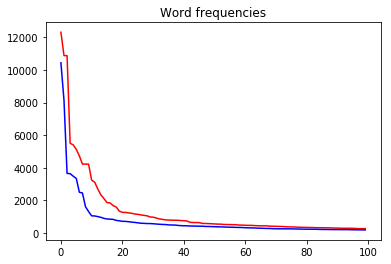
\includegraphics[width=0.75\textwidth]{pics/word_frequencies}
  \caption{Word Frequencies on ConLL-2003 and NER-on-HTML}
  \label{fig:word_frequencies}
\end{figure}

\begin{table}[h]
  \small
  \begin{center}
    \begin{tabular}{ llll }
      \toprule
      Word & Frequency & Word & Frequency \\
      \midrule
      the & 12310 & , & 10439      \\
      , & 10876 & - & 8140         \\
      . & 10874 & ) & 3655         \\
      of & 5502 & ( & 3641         \\
      in & 5405 & : & 3484         \\
      to & 5129 & of & 3345        \\
      a & 4731 & and & 2499        \\
      ( & 4226 & professor & 2456  \\
      ) & 4225 & university & 1611 \\
      and & 4223 & research & 1315 \\
      \bottomrule
    \end{tabular}
  \end{center}
  \caption{Thirty most frequent words for the ConLL-2003 dataset and the NER-on-HTML dataset}
  \label{tab:conll}
\end{table}

The word frequency distributions for the hundred most frequenct words in both datasets 
are described in Figure~\ref{fig:word_frequencies}. Their shape is rather similar, 
presenting a small number of very frequent words and a long tail of words that happen 
only once or twice in the dataset. This long tail is where most named entities are located.
To allow further comparison between both datasets, we present the ten most frequent words 
(including punctuation signs) for each dataset in Table~\ref{tab:frequent_words}. As 
expected, the ConLL-2003 contains more generic terms whereas the subject of the NER-on-HTML
becomes evident with words such as "professor" and "university" happening with a high
frequency in the corpus. Also, punctuation signs are relatively more frequent in the 
NER-on-HTML owing to the factual tabular structure of the HTML texts present in the 
collection. 

\section{Dictionary}

\begin{table}[h]
  \small
  \begin{center}
    \begin{tabular}{ lllll }
      \toprule
      Data file & Precision & Recall & F1 & Correct names \\
      \midrule
      Training   & 0.7316 & 0.2303 & 0.3504 & 1341 of 5822 \\ 
      Validation & 0.8474 & 0.2858 & 0.4274 & 511 of 1788 \\ 
      Test       & 0.8717 & 0.3287 & 0.4773 & 890 of 2708 \\ 
      \bottomrule
    \end{tabular}
  \end{center}
  \caption{Gazetteer coverage in each data file}
  \label{tab:gazetteer}
\end{table}

A dictionary or gazetteer can be a powerful aid on generic sequence labeling systems,
eventhough deep learning architectures can be much less reliant on these types of 
features, especially when we make use of pretrained word embeddings. We extracted 
a list of 1,595,771 researcher names from the DBLP database and annotated tokens in the
NER-on-HTML dataset with exact and partial matches tags. That is, if a sequence of tokens
corresponded exactly to a name from the DBLP list, the entire sequence was annotated as 
an exact match. Otherwise, if some tokens in the sequence matched a name from the DBLP
list partially, the matching tokens were annotated with a partial match tag. 
Table~\ref{tab:gazetteer} shows the precision, recall and F1 scores obtained with an
exact gazetteer matching strategy in each NER-on-HTML data file as a baseline. This is 
the performance obtained by only extracting sequences of tokens that correspond to an exact 
match with the DBLP list. As expected, recall is very low and precision falls short of
top performance extraction methods. Having established this baseline, any useful extraction 
method should easily beat the dictionary exact matching approach.

\section{Features}

Finally, thirteen categorical features were associated with each token in the dataset. 
These were selected through feature engineering from a larger pool of features, 
considering their aid to the performance of the extraction systems. Deep learning 
architectures can work incredibly well without any of these features, however these 
features are of critical importance to classical approaches such as HMMs and CRFs. 
The selected features are presented in Table~\ref{tab:features}. Additionaly, all 
models also make use of the unmodified tokens as features directly or as embedding
lookups.

\begin{table}[h]
  \small
  \begin{center}
    \begin{tabular}{ ll }
      \toprule
      Feature & Description \\
      \midrule
      1  & Unaccented lowercase token \\
      2  & Exact gazetteer match \\
      3  & Partial gazetteer match \\
      4  & Log name gazetteer count\\
      5  & Log word gazetteer count\\
      6  & Email \\
      7  & Number \\
      8  & Honorific (Mr., Mrs., Dr., etc.)\\
      9  & URL \\
      10 & Is capitalized \\
      11 & Is a punctuation sign \\
      12 & HTML tag + parent \\
      13 & CSS class \\
      \bottomrule
    \end{tabular}
  \end{center}
  \caption{Features used in the NER-on-HTML dataset}
  \label{tab:features}
\end{table}

Feature 1 represents the token converted to unaccented lowercase format.
Feature 2 represents an exact match of a sequence of tokens to any of the 1,595,771 
names from the DBLP list, and feature 3 represents a partial match. Feature 4 is the rounded logarithm of 
the frequency of a token in the gazetteer, and feature 5 is the rounded logarithm of the frequency
of a token in a word corpus obtained through a random crawl on university websites.
Features 6 to 11 represent a simple regular expression match to an email, number, 
honorific, URL, capitalization or punctuation sign. Feature 12 represents the HTML enclosing tag 
and its parent concatenated. Finally, feature 13 represents all CSS classes concatenated. 
Features 12 and 13 are of importance to the self-training strategy of HMMs described in 
Section~\ref{sssec:self_training} and the attention architecture for DNNs described in
Section~\ref{sssec:attention}.


\chapter{Sequence Labeling Methods for Named Entity Recognition}

Many important tasks in Natural Language Processing ranging from Part-of-speech 
tagging to Named Entity Recognition involve attributing labels to sequences of 
words. In the \textit{Named Entity Recognition} task, we want to 
attribute labels to tokens, classifying them into one of many predefined classes 
according to the available evidence. In Part-of-speech tagging we do essentialy
the same task with different classes.
Both of these tasks, as any other sequence labeling task can be modeled generically.
If $ X = \{x_1, x_2, ..., x_n\} $ is a sequence of words and 
$ Y = \{y_1, y_2, ..., y_n\} $ is a sequence of labels attributed to the word 
sequence $ X $. Our goal is to find the optimal sequence of labels $ Y* $
that maximizes the conditional probability of $ Y $ given $ X $. That is:

\begin{equation}
Y^* = \argmax_{Y} P(Y|X)
\end{equation}

Calculating these probabilities precisely is impractical due to the exponential
increase in the number of label combinations as we increase the sequence size 
$ n $. As $ n $ becomes large, label combinations will become increasingly
uncommon in the dataset, what will make probability estimation less reliable.
Taking this into consideration, ultimately, the difference between sequence 
labelling models lies in the assumptions behind the estimation of the conditional 
probabilities $ P(Y|X) $. In this chapter we will describe several machine learning
approches to sequence labeling, starting with the classical methods in 
Section~\ref{sec:classical_methods}, which are: Hidden Markov Models, 
Conditional Random Fields and Maximum Entropy Markov Models. In 
Section~\ref{sec:neural_models} we will describe some neural architectures for 
sequence labelling, which are: bidirectional recurrent neural networks, LSTM-CRF,
CNN character representations, LSTM character representations.
Finally, in Section~\ref{sec:word_embeddings} we will describe how word embeddings can
help improve the performance of some of the previously introduced sequence labeling 
methods on the Named Entity Recognition for the web task.

\section{Classical Methods}

\subsection{Hidden Markov Models}

A Markov Model is a stochastic model that computes the most probable sequence of states 
given a limited set of observable states $ S = \{s_1, s_2, ..., s_n \} $.
The Hidden Markov Model (HMM) differs from the Markov Model in that it
does not observe the states directly, but rather a probabilistic function of those 
states. For example in NER, the words are observed, however the Named Entity labels
associated with these words are not. Formally, we want to compute the most probable
sequence of labels $ Y = \{y_1, y_2, ..., y_n\} $ for a sequence of observed tokens
$ X = \{x_1, x_2, ..., x_n\} $.

\begin{equation}
Y^* = \argmax_{Y} P(Y|X)
\end{equation}

With Bayes theorem, we can write $ P(Y|X) $ as:

\begin{equation}
P(Y|X) = \frac{P(X|Y) P(Y)}{P(X)}
\end{equation}

Since $ P(X) $ is the same for all label sequences $ Y $, we can simply maximize
the probability $ P(X|Y) P(Y) $.

A HMM makes two assumptions. First, the probability of being in a given state depends 
only on a fixed number of previous states. That is:

\begin{equation}
P(y_i|y_{i-1}x_{i-1}, y_{i-2}x_{i-2}, ..., y_1x_1) = P(y_i|y_{i-1}, y_{i-2},..., y_{i-k})
\end{equation}

In fact, we can get much better results on the NER task by looking at trigrams
or quadrigrams ($ k = 2 $ or $ k = 3 $) instead of bigrams as with a regular HMM. 
Some label assignments are highly improbable, such as single token named entities 
separated by a common word. These kinds of patterns can be perceived by a higher order HMM.
Second, the probability of a word depends only on its assigned label. That is:

\begin{equation}
P(x_i|y_{i-1}x_{i-1}, ..., y_1x_1) = P(x_i|y_i)
\end{equation}

With these assumptions, 
the probability $ P(Y|X) $ can be approximated by the expression:

\begin{equation}
P(Y|X) \propto \prod_{i=k+1}^{n} P(y_i|y_{i-1}, y_{i-2}, ..., y_{i-k}) P(x_i|y_i)
\end{equation}

All relevant probabilities can be estimated through maximum likelihood estimation from the relative
frequencies of labels and features in the corpus. The best sequence of labels can be computed 
with a variable state Viterbi approach \cite{Li2000}. However, as we increase $ k $, this computation 
becomes exponentially more expensive. The beam-search strategy may be employed for a faster 
search, but we found that for $ k \leq 4 $, the Viterbi algorithm is still viable.

HMM based taggers have been successfully applied in many NLP and WDE tasks 
\cite{Rabiner1990,Leek1997,Freitag2000}. They are incredibly fast to train and also they are very 
interpretable, making them a good choice for a first approximation. However, these models 
are highly dependent on the right selection of features, what may outweigh the benefit of a 
small training cost.

\subsection{Self training} 
\label{sssec:self_training}

In the task of NER on HTML, there are useful features related to the HTML
structure that can help in identifying named entities. In a given website, named
entities tend to occur inside the same HTML tags. The HTML tag feature or other
HTML features could easily be incorporated in the HMM. However, these 
features are only useful inside a single website and they cannot be generalized, 
because different websites use distinct HTML templates. 
Therefore, we propose a self-training strategy to obtain probabilities for
these HTML features. It is implemented like this:

\begin{itemize}
\item Train the HMM without any HTML features.
\item Compute labels for a website with the trained HMM.
\item Use the computed labels as a proxy for the actual labels in the 
website and estimate HTML feature frequencies for this website alone.
\item Recompute the labels now using the HTML feature probabilities.
\end{itemize}

In theory, this strategy could be used with any sequence tagger, however
retraining a classifier with new features can become prohibitively expensive.
This strategy is only possible because the computation of HTML feature
frequencies can be performed very quickly. This adds very little overhead 
to the original HMM and improves precision and recall by a considerable 
margin.

\subsection{Linear Chain Conditional Random Fields}

A Linear Chain Conditional Random Field (CRF) is the discriminative analog to the HMM,
it was first introduced by Lafferty \cite{Lafferty2001}. It is a distribution $ P(Y|X) $ that takes the form:

\begin{equation}
P(Y|X) = \frac{1}{Z(x)} \prod_{t=1}^{T} exp \left( \sum_{k=1}^{K} \theta_k f_k(y_{t-1}, y_t, X) \right)
\end{equation}
\\

where $ \theta $ is the parameter vector that we are going to learn, $ f_k(y_{t-1}, y_{t}, X) $ 
are feature functions over the current timestep $ t_y $, the previous timestep $ y_{t-1}$, 
and the observation vector $ X $. And the partition function $ Z(x) $, takes the form:

\begin{equation}
Z(x) = \sum_{Y} \prod_{t=1}^{T} exp \left( \sum_{k=1}^{K} \theta_k f_k(y_{t-1}, y_t, x) \right)
\end{equation}
\\

which is a sum over all possible label assignments $ Y $. The partition function can be efficiently
and exactly calculated with the sum-product algorithm. Parameter estimation is usually done through 
negative log likelihood minimization. The function can be optimized with techniques suitable for other 
maximum entropy models such as L-BFGS \cite{Liu1989}. The most likely label sequences can be decoded 
with the Viterbi algorithm, as was the case for HMMs.

CRFs are more general than HMMs because the transitions from $ y_{t-1} $ to $ y_{t} $ can depend 
on the whole vector of observations $ X $. This flexibility of feature functions allows for a wide range of
possibilities. Recently, CRFs have been successfully employed as the output layer in complex neural 
architectures bringing improvements over models that compute labels independently.

\section{Neural Network Architectures}

Recurrent neural networks (RNN) have been successfully employed on numerous NLP tasks such as
language modelling, POS tagging, speech recognition and NER. Different from feed-forward 
neural networks, RNNs can retain information in their internal state, making them more 
suitable for processing sequences, and consequently for solving text related tasks. 
Figure~\ref{fig:rnn_network} describes an RNN for sequence labeling unrolled through multiple 
timesteps. 

\begin{figure}[h]
  \centering
  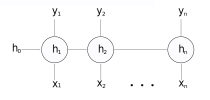
\includegraphics[width=0.75\textwidth]{pics/rnn_network}
  \caption{RNN for NER}
  \label{fig:rnn_network}
\end{figure}

At each timestep, the neural network computes a hidden state $ h_t $ using an input 
vector $ x_t $ and the previous hidden state $ h_{t-1} $, that retains information from past 
iterations. Finally, the RNN produces an output vector $ y_t $ representing the label for that 
timestep. A common definition for an RNN cell is given by the equations:

\begin{flalign*}
h_t &= tanh(W_x x_t + W_h h_{t-1}) &\\
y_t &= softmax(W_y h_t) &
\end{flalign*}

Where $ W_x $, $ W_h $ and $ W_y $ are weight matrices that can be trained with the 
Backpropagation Through Time (BPTT) algorithm. Theoretically, RNNs are capable of learning
and retaining long term dependencies through their internal state $ h_t $. However, in practice,
it becomes difficult due to the vanishing gradient problem. Long short term memory networks (LSTM) were 
introduced by Hochreiter and Schmidhuber \cite{Hochreiter1997} with this problem in mind and 
have been popularized since then. 

LSTMs incorporate a memory cell $ c $ in the RNN definition and three gates to control 
the flow of information that comes in and out of the memory cell.
The input gate $ \Gamma_{i} $ controls the amount of new information that will flow into the memory cell,
the forget gate $ \Gamma_{f} $ controls the amount of previous information that will be retained in the memory
cell, and the output gate $ \Gamma_{o} $ controls the amount of information stored in the memory cell that
will be used to compute the output activation of the LSTM unit. 
LSTM cell implementations vary slightly in the literature. A visual description of 
our LSTM cell is provided in Figure~\ref{fig:lstm_cell}.

\begin{figure}[h]
  \centering
  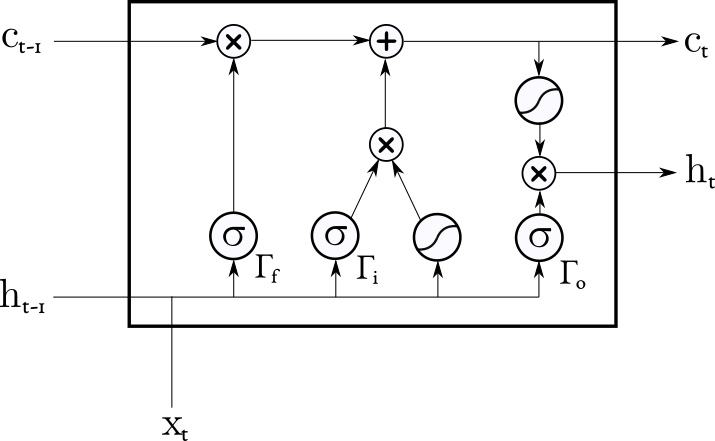
\includegraphics[width=0.75\textwidth]{pics/lstm_cell}
  \caption{LSTM Cell}
  \label{fig:lstm_cell}
\end{figure}

The equations for the LSTM cell are:

\begin{flalign*}
\Gamma_{i} &= \sigma(W_i \cdot [x_t,h_{t-1}] + b_i) &\\
\Gamma_{f} &= \sigma(W_f \cdot [x_t,h_{t-1}] + b_f) &\\ 
\Gamma_{o} &= \sigma(W_o \cdot [x_{t},h_{t-1}] + b_o) &\\
c_t        &= \Gamma_{f} \ast c_{t-1} + \Gamma_{i} \ast tanh(W_c \cdot [x_{t},h_{t-1}] + b_c) &\\
h_t        &= \Gamma_{o} \ast tanh(c_t) &
\end{flalign*}

Where $ \sigma $ is the logistic sigmoid function. $ \Gamma_i $, $ \Gamma_f $, and $ \Gamma_o $ are the input,
forget and output gates, respectively, and $ W_i $, $ W_f $, $ W_o $ are the weight 
matrices corresponding to each gate. $ c_{t} $ is the cell 
state at time $ t $ and $ h_{t} $ is the hidden state at time $ t $. 
The vector $ [x_{t},h_{t-1}] $ is formed by concatenating the current input vector 
$ x_{t} $ and the hidden vector from a previous timestep $ h_{t-1} $. Finally,
$ A \ast B $ represents the element-wise multiplication of matrices $ A $ and $ B $
and $ A \cdot B $ represents the dot product of $ A $ and $ B $.

This implementation differs from the LSTM cell described in Huang et al. \cite{Huang2015}
in that the gates $ \Gamma_i $ and $ \Gamma_f $ do not receive inputs from the previous 
cell state $ c_{t-1} $ and the output gate $ \Gamma_{o} $ does not receive inputs from the current cell 
state $ c_{t} $. This variation produces little difference in terms of model accuracy on
the performed task, but it reduces model complexity.

\subsection{BI-LSTM-CRF}
\label{sssec:lstm_crf}

On named entity recognition tasks, both past and future words are important 
to attribute a label at time $ t $, however a regular LSTM network only takes 
past states into consideration. A bidirectional LSTM solves this problem by stacking 
two regular LSTMs, and feeding them with observations in opposite directions. The first LSTM 
receives forward states and the second LSTM receives backward states. The hidden states from both 
networks can then be concatenated at each timestep to produce output labels. With this 
architecture, LSTM cells may use information from past and future timesteps to decide 
the label at time $ t $.

Huang et al. \cite{Huang2015} proposed a bidirectional LSTM with a CRF layer (BI-LSTM-CRF) on 
the output to tackle the sequence tagging problem. The main benefit of adding a CRF layer 
in the neural sequence model is that the labels are jointly decoded for a whole sentence 
instead of being predicted individually. Another possibility would be to use a beam search
decoder to find an optimal sequence of labels. Predicted tags should be highly correlated 
in a named entity recognition task, so it is desirable to predict sequences conjointly.
The BI-LSTM-CRF is described in Figure~\ref{fig:bi_lstm_crf}.

\begin{figure}[h]
  \centering
  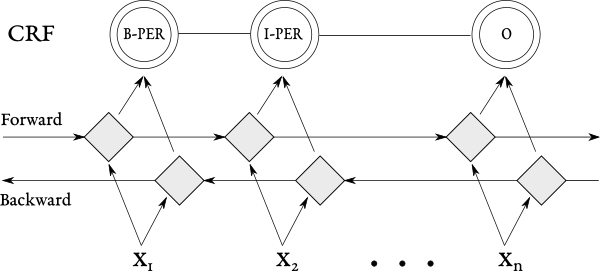
\includegraphics[width=0.75\textwidth]{pics/bi_lstm_crf}
  \caption{Bidirectional LSTM-CRF}
  \label{fig:bi_lstm_crf}
\end{figure}

This architecture achieved an F1 score of 90.10 on the English data from the CoNLL-2003 
NER shared task \cite{Sang2003}, in contrast to 85.17 for a bidirectional LSTM without 
a CRF layer. 
In our experiments, the LSTM-CRF architecture uses a bidirectional LSTM with 100 
hidden states, no peepholes and input and output dropout layers with a dropout
rate of 0.5. The dropout layers have proven to be very important to prevent overfitting 
and allow better generalization.

\subsection{CNN character representations}
\label{sssec:lstm_crf_cnn}

Ma and Hovy \cite{Ma2016} proposed to add a convolutional neural network (CNN) layer 
on top of a bidirectional LSTM-CRF to encode character-level information. The CNN
layer is described visually in Figure \ref{fig:cnn}.

\begin{figure}[h]
  \centering
	  \includegraphics[width=0.75\textwidth]{pics/cnn}
  \caption{CNN based character representations}
  \label{fig:cnn}
\end{figure}

The convolutional neural network receives character embeddings as inputs. The character 
representations generated by the CNN are combined with word level representations 
and fed to the BI-LSTM-CRF described in section \ref{sssec:lstm_crf}.
This architecture can learn morphological features that are very
useful in the NER task, since similar named entities often present morphological similarities. 
This architecture obtained an F1 score of 91.21 in the CoNLL2003 dataset. In our experiments, 
the LSTM-CRF architecture with CNN character representations uses a one dimensional convolutional 
neural network with 30 filters and a window size of three characters on top of the LSTM-CRF 
architecture. The character embeddings fed to the CNN have 30 dimensions that are randomly 
initialized.

\subsection{LSTM character representations}

Lample et al \cite{Lample2016} proposed to use a bidirectional LSTM to model character-level 
representations on top of a BI-LSTM-CRF. Combining the forward and backward LSTM hidden states 
to form the character representation, as described in Figure~\ref{fig:lstm_char}. 

\begin{figure}[h]
  \centering
  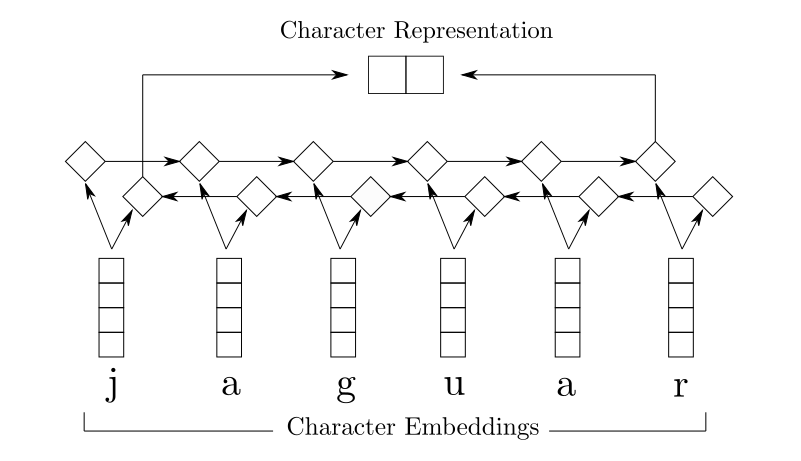
\includegraphics[width=0.75\textwidth]{pics/lstm_char_representations}
  \caption{LSTM based character representations}
  \label{fig:lstm_char}
\end{figure}

This character representation is also combined with a word 
representation and fed to a BI-LSTM-CRF network. 
The forward state is expected to be a better representation of the suffix of 
a token, and the backward state is expected to be a better representation of 
the prefix of a token. This differentiates the architecture
from the CNN based approach described in Section~\ref{sssec:lstm_crf_cnn}, because CNN filters 
discover positional invariant features, while LSTMs can better represent 
suffixes and prefixes. In our experiments, 
the LSTM-CRF architecture with LSTM character representations was implemented with a bidirectional 
LSTM with 25 hidden states, producing character representations of 
size 50. The character embeddings have 30 dimensions that are randomly initialized.

\subsection{Network training}

All neural models were trained using mini batch Stochastic Gradient Descent over 50 epochs with batch size 10,
learning rate 0.01, momentum 0.9 and decay rate 0.05. We used early stopping \cite{Caruana2000} to select the best 
parameters, considering the F1 measure in the validation set. All neural models used 
GloVe 100-dimensional word embeddings \cite{Pennington2014} that were fine tuned during training.
In the case of NER on HTML, word embeddings work similarly to a gazetteer. Named entities 
with the same type have similar embeddings, so good word embeddings can achieve exceptional 
performance with little training and without a gazetteer. 

\section{Word Embeddings}

\subsection{Word2Vec}

\subsection{Glove}

\subsection{Elmo}

\subsection{Other embeddings and some thoughts}

BERT, language model do Chen. How a human can never learn with so many words.

\section{Numerical Optimization}

How to do it? ADAM. SGD. Minibatch.

\chapter{Sequence Labeling on HTML}

Self training for HMMs

Soft attention

Hard attention

F1 optimization

\chapter{Experiments}

We conducted experiments to evaluate sequence labeling methods of named entity 
recognition on HTML in the context of Web data extraction using the dataset 
described in Section~\ref{sec:ner_dataset}. The tested models are described in
Table~\ref{tab:models}.

\begin{table}[h]
  \small
  \begin{center}
    \begin{tabular}{ ll }
      \toprule
      Model & Description \\
      \midrule
      hmm-1            & Regular HMM \\
      hmm-2            & HMM with $ k=2 $ \\
      hmm-3            & HMM with $ k=3 $ \\
      crf              & Linear chain conditional random fields \\
      bi-lstm-crf      & BI-LSTM-CRF model \\
      bi-lstm-crf-cnn  & BI-LSTM-CRF with CNN character representations \\
      bi-lstm-crf-lstm & BI-LSTM-CRF with LSTM character representations \\
      \bottomrule
    \end{tabular}
  \end{center}
  \caption{Model descriptions}
  \label{tab:models}
\end{table}

The evaluation of model performance was done through the precision, recall and 
F1 scores \cite{Rijsbergen1979}. Precision is the percentage of named entities found by 
the model that are correct. Recall is the percentage of named entities that are present
in the corpus and were found by the model. The F1 score is a composite measure that combines
precision and recall with the formula:

\begin{equation}
F1 = \frac{2 * precision * recall}{precision + recall}
\end{equation}

Named entities were only considered to be correct if they were a complete match of the 
corresponding entity in the dataset.

\section{Experiment 1: No features}

Experiment 1 aimed to evaluate the performance of sequence model with no features
besides GloVe-100 embeddings. In the case of HMMs, only the lowercase
unaccented token was used as a feature. Table \ref{tab:experiment1} 
shows the Precision (P), Recall (R), and F1-scores (F1) for this
experiment.

\begin{table}[h]
  \small
  \begin{center}
    \begin{tabular}{ lllllll }
      \toprule
      \multirow{2}{*}{Model} & \multicolumn{3}{c}{Validation} & \multicolumn{3}{c}{Test} \\
                             & \multicolumn{1}{c}{P} & \multicolumn{1}{c}{R} & \multicolumn{1}{c}{F1}
                             & \multicolumn{1}{c}{P} & \multicolumn{1}{c}{R} & \multicolumn{1}{c}{F1} \\
      \midrule
      hmm-1	       & 0.6965 & 0.5749 & 0.6299 & 0.6263 & 0.4431 & 0.5190 \\
      hmm-2	       & 0.7047 & 0.6286 & 0.6645 & 0.6480 & 0.5222 & 0.5783 \\
      hmm-3	       & 0.6127 & 0.6141 & 0.6134 & 0.5471 & 0.4634 & 0.5018 \\
      crf	       & 0.7173 & 0.6683 & 0.6920 & 0.6671 & 0.5868 & 0.6244 \\
      bi-lstm-crf      & 0.8484 & 0.9044 & 0.8755 & 0.8358 & 0.8497 & 0.8427 \\
      bi-lstm-crf-cnn  & 0.9058 & 0.9575 & 0.9309 & 0.8779 & 0.8737 & 0.8758 \\
      bi-lstm-crf-lstm & 0.9134 & 0.9435 & 0.9282 & \textbf{0.8920} & \textbf{0.8815} & \textbf{0.8867} \\
      \bottomrule
    \end{tabular}
  \end{center}
  \caption{Precision, recall and F1 in the NER on HTML dataset for models that incorporate no features}
  \label{tab:experiment1}
\end{table}

Without carefully designed features or gazetteers, HMMs and CRFs have a very 
poor performance, achieving an F1-score of only 0.5783 for HMM-2 and 0.6244 for CRF
at the test set. This is expected, since these models rely on good feature selections.

The neural models achieved high F1-scores in the test
set even with the absence of features. The plain BI-LSTM-CRF architecture improved performance 
significantly in comparison with the conventional CRF (0.8427 against 0.6244). 
Also, neural character representations boosted performance by a significant margin
reaching an F1-score of 0.8758 for CNN-based representations and 0.8867 for LSTM-based
representations. LSTM based representations were superior in modelling
morphological features, perhaps because they are able to differentiate suffixes 
and prefixes, while CNN filters are position invariant. 

The results in Experiment 1 also show that pretrained word embeddings can work 
as a kind of universal gazetteer. Words with similar embeddings are likely to 
belong to the same class. This knowledge combined with the ability to learn 
morphological features can make up for the scarcity of textual data on some 
webpages.

\section{Experiment 2: All features}

Experiment 2 aimed to evaluate the performance of sequence model with all
the features described in Table~\ref{tab:features}. In this experiment, we
also evaluate the self-training strategy for HMMs described in Section 
\ref{sssec:self_training}. The self trained HMMs are described with the 
suffix "+ST". Table \ref{tab:experiment2} shows the results for Experiment 2.

\begin{table}[h]
  \small
  \begin{center}
    \begin{tabular}{ lllllll }
      \toprule
      \multirow{2}{*}{Model} & \multicolumn{3}{c}{Validation} & \multicolumn{3}{c}{Test} \\
                             & \multicolumn{1}{c}{P} & \multicolumn{1}{c}{R} & \multicolumn{1}{c}{F1}
                             & \multicolumn{1}{c}{P} & \multicolumn{1}{c}{R} & \multicolumn{1}{c}{F1} \\
      \midrule
      hmm-1	         & 0.6061 & 0.7282 & 0.6616 & 0.7106 & 0.7633 & 0.7360 \\
      hmm-2	         & 0.6279 & 0.7550 & 0.6856 & 0.7521 & 0.7810 & 0.7663 \\
      hmm-3	         & 0.6573 & 0.7819 & 0.7142 & 0.7523 & 0.7795 & 0.7657 \\
      hmm-1+ST           & 0.7032 & 0.9077 & 0.7925 & 0.7522 & 0.8663 & 0.8052 \\
      hmm-2+ST           & 0.7321 & 0.9172 & 0.8143 & 0.7737 & 0.8789 & 0.8230 \\
      hmm-3+ST           & 0.7551 & 0.9172 & 0.8283 & 0.7961 & 0.8534 & 0.8237 \\
      crf	         & 0.9024 & 0.9049 & 0.9037 & 0.8751 & 0.8227 & 0.8481 \\
      bi-lstm-crf        & 0.9430 & 0.9530 & 0.9480 & 0.8998 & 0.8527 & 0.8756 \\
      bi-lstm-crf-cnn    & 0.9244 & 0.9715 & 0.9474 & 0.9017 & \textbf{0.8973} & \textbf{0.8995} \\
      bi-lstm-crf-lstm   & 0.9465 & 0.9692 & 0.9577 & \textbf{0.9108} & 0.8715 & 0.8907 \\
      \bottomrule
    \end{tabular}
  \end{center}
  \caption{Precision, recall and F1 in the NER on HTML dataset for models that incorporate all features}
  \label{tab:experiment2}
\end{table}

Conventional models like HMMs, and CRFs can become competitive with
the right selection of features and a good gazetteer, however they still lose
to the best neural model without features, demonstrating their inherent limitations.
HMMs that employed trigrams or quadrigrams (hmm-2, hmm-3) performed better than
regular HMMs. Also, we can see that the self-training strategy for HMMs improved 
the quality of the models significantly in all cases, boosting both precision and recall. 
This hints at the possibility to adapt this strategy to neural networks and boost
the performance of neural models on the NER on HTML task.

The neural models also improved a little with the addition of features. The plain BI-LSTM-CRF
model gets a closer performance to the models that employed neural character 
representations. It suggests that the LSTM and CNN character representations 
were able to learn at least part of the morphological features automatically in the
first experiment. So, when these features are added explicitly, the differences 
in performance between different neural models become less noticeable.


\chapter{Related Work}

% Getting simple structured information out of text.

In the last 20 years, the astonishing growth of public information in the Web has 
led to the development of a number of different approaches to the problem of Web 
data extraction. Traditionally, the task was solved by designing special purpose
programs called wrappers to recognize relevant data and store records in a structured
format. These early tools varied wildly relative to their degree of automation. 

It was readily perceived that manual wrapper generation was a rather tedious and
error prone process, unsuited for large scale operations. Wrappers tend to
break frequently because they rely heavily on webpage features that can change 
often. So, in the late nineties, several authors advocated for wrapper induction, a technique 
that consists of automatically constructing wrappers from a small set of examples by 
identifying delimiters or context tokens that single out the desired attributes. 
Some remarkable wrapper induction methods are WIEN \cite{Kushmerick2000}, Soft 
Mealy \cite{Hsu1998} and STALKER \cite{Muslea1999}.

Despite being better than constructing wrappers manually, wrapper induction methods 
still suffered from a lack of expressive power and flexibility. These methods had 
trouble handling records with missing attributes or unusual structures because
patterns could only be identified if they happened at least once in the examples.

Other approaches such as NoDoSE \cite{Adelberg1998} and Debye \cite{Laender2002a} 
brought greater flexibility to wrapper induction methods by requiring a greater level 
of human interaction through graphical user interfaces. Web data extraction techniques often 
require some sort of assistance from human experts to boost accuracy. One of the main challenges 
in the field lies in determining an adequate trade-off between the degree of automation and 
the precision and recall of the data extraction tool.

To automate the task of Web data extraction completely some approaches,
such as Road Runner \cite{Crescenzi2001}, removed entirely the need for data examples.
Road Runner parses documents belonging to a same class (e.g. books on Amazon) and 
generates wrappers based on their similarities and differences, yielding comparable results 
to those obtained by wrapper induction methods. However, like previous approaches, it was 
unsuited for cross site extraction tasks because the learned rules were not general enough.

NLP based approaches aimed at extracting more general rules that could possibly
be employed over multiple websites. RAPIER \cite{Califf1999} is a method of rule
extraction that uses information such as part-of-speech tags and semantic classes from
a lexicon to derive patterns from a set of training examples. This approach is more
flexible than the wrapper induction methods, however it achieves much lower rates of 
recall and precision.

In 2002, a survey by Laender et al. \cite{Laender2002} made a thorough classification of the
early approaches with a taxonomy based on their main technology, being them: languages for
wrapper development, HTML-aware tools, NLP-based tools, Wrapper Induction Tools,
Modeling-based tools and Ontology-based tools. Some noteworthy examples from this era
are: 

\begin{itemize}
\item TSIMMIS \cite{Hammer1997} and WebOQL \cite{Arocena1999}, which are special purpose 
languages for building wrappers.

\item Road Runner \cite{Crescenzi2001}, XWRAP \cite{Liu2000} and W4F \cite{Sahuguet1999}, 
which are HTML-aware tools that infer meaningful patterns from the HTML structure.

\item RAPIER \cite{Califf1999}, SRV \cite{Freitag1998}, WHISK \cite{Soderland1999}, which 
are NLP-based tools.

\item WIEN \cite{Kushmerick2000}, Soft Mealy \cite{Hsu1998} and STALKER \cite{Muslea1999} which 
are wrapper induction methods.

\item NoDoSE \cite{Adelberg1998} and Debye \cite{Laender2002a}, which are semi supervised modeling
based tools that require some interaction with the user by means of a graphical
user interface.
\end{itemize}

In 2006, Chang et al. \cite{Chang2006} complemented the previous surveys with semi-supervised 
technologies such as Thresher \cite{Hogue2005}, IEPAD \cite{Chang2001} and 
OLERA \cite{Chang2004}. They differed from supervised 
and unsupervised methods because they either needed only a rough description of
data from users for extraction rule generation or some level of post processing
that needed user attention. The survey also mentioned newer unsupervised methods
such as DeLa \cite{Wang2003}, Exalg \cite{Arasu2003} and Depta \cite{Zhai2005}.

Most of the early information extraction systems were rule-based with either 
manual rule description or automatic rule learning from examples, thus they
suffered from a lack of flexibility when dealing with noisy and unstructured data.
Huge progress in the field of statistical learning led to the development of
statistical models that tried to solve this problem.

In 2008, Sarawagi \cite{Sarawagi2008} produced a survey that classified wrappers into
rule-based methods, statistical methods and hybrid models, bringing together 
the fields of named entity recognition, relationship extraction and information extraction. 
The rule based methods encompass most of the 
previous models. The statistical methods convert the extraction task into a token labeling 
task, identifying the target entities through the assignment of labels as in a typical 
Named Entity Recognition task. Traditionally, Hidden Markov Models \cite{Leek1997,Freitag1999}, 
Linear Chain Conditional Random Fields \cite{Lafferty2001}, and Maximum Entropy Taggers 
\cite{McCallum2000} have been the usual choice for linear sequence tagging models.
More recently, with the advancement of Natural Language Processing and Deep Learning, 
neural models outperformed previous NER methods for plain text. Huang et. al. \cite{Huang2015} introduced the 
bidirectional Long Short-Term Memory (LSTM) model with a Conditional Random Field (CRF) output layer
for NER. Ma and Hovy \cite{Ma2016} incorporated Convolutional Neural Network based character representations 
on top of the architecture. And Lample et. al. \cite{Lample2016} introduced
LSTM based character representations. 

Surveys by Ferrara et al. \cite{Ferrara2014}, Schulz et al. \cite{Schulz2016} and 
Varlamov et al. \cite{Varlamov2016} updated the previous surveys on information 
extraction methods with some interesting innovations. 
Some examples are: the Visual Box Model \cite{Krupl2005}, a data extraction system that produces 
a visualization of the webpage to exploit visual cues to identify data presented in a tabular form;
automatic wrapper adaptation \cite{Ferrara2011}, a technique that tries to reduce the cost of 
wrapper maintenance by measuring the similarity of HTML trees and adapting
wrappers to the new page structure; AutoRM \cite{Shi2015}, a method to mine
records from a single webpage by identifying similar data regions through DOM
tree analysis; Knowledge Vault \cite{Dong2014}, a method that combines different 
extraction approaches to feed a probabilistic knowledge base.

Most data extraction systems focus on extracting information from single websites
and are therefore unsuited for cross website extraction tasks. Even unsupervised
approaches that are domain independent, such as RoadRunner \cite{Crescenzi2001} 
and EXALG \cite{Arasu2003} only work well for extracting data from pages generated 
from a same template. 

A statistical approach to unsupervised domain 
independent Web data extraction was described by Zhu et al \cite{Zhu2005}. The 2D CRF 
model takes a webpage segmented into data blocks and employs a two dimensional conditional 
random field model to perform attribute labeling. The model was further improved
\cite{Zhu2006} to model record segmentation and attribute labeling as a joint task.
Some of the limitations of early unsupervised methods 
were also tackled by ObjectRunner \cite{Abdessalem2010} and AMBER \cite{Furche2012}. 
These methods work by annotating webpages automatically with regular expressions, gazetteers and 
knowledge bases. They can rectify low quality annotations and even improve the annotators
by exploring regular structures in the DOM during the record segmentation phase.

Web data extraction methods have undoubtedly improved extraordinarily, but
as pointed by Schulz et al. \cite{Schulz2016}, it is difficult to compare the results 
achieved by competing tools, and many seem to rely excessively on heuristic methods.
In that regard, the recent advancements in sequence taggers may provide more robust and
flexible extraction tools.


\chapter{Conclusion}

Machine-learning-based sequence labeling models provide a flexible approach to Web data 
extraction, in contrast to more traditional methods. In simple cases, a neural
named entity tagger may be sufficient to solve the entire data extraction task. In 
other cases, the sequence tagger remains an important part of the web data extraction
system, as it performs attribute labeling on data records with accuracy and flexibility.

In this article, we compared the performance of different sequence models on the task of
named entity recognition on HTML, introducing a novel dataset that is publicly available. 
We found that there are two components to the most successful models: neural based character 
representations that extract morphological features automatically, and the joint modelling 
of output labels.

We showed that a BI-LSTM-CRF neural network with LSTM-based character representations can 
be employed effectively to solve a web data extraction task, achieving an F1-score of 
0.8867 with no feature engineering on the faculty listings dataset.

The effective recognition of named entities on HTML is an essential step in most general 
Web data extraction methods. The accuracy achieved by deep neural architectures even
on webpages that are very different from the plain text for which these architectures 
were initially designed shows the potential for a truly flexible approach to cross domain 
web data extraction.


\ppgccbibliography{bibfile}


\begin{appendices}
\label{app:html_segmenter}

\chapter{HTML sentence segmenter}

Lorem ipsum dolor.

% \chapter{Outro ap�ndice}
% 
% \dummytxta
% 
\end{appendices}
% 
% 
% \begin{attachments}
% 
% % Para cada anexo, um \chapter
% \chapter{Um anexo}
% 
% \dummytxta
% 
% \chapter{Outro anexo}
% 
% \dummytxta
% \end{attachments}


\end{document}
